\chapter{Resultat}
\label{cha:results}

\section{Systembeskrivning - vidareutveckling av TreeD}
%% Översiktlig beskrivning system, dokument
%% Vad har kunden för värde hos det som skapats?

Nedan följer en beskrivning av det ROS-baserade system som byggde vidare på TreeD och som utvecklades innan kraven i projektet omförhandlades med kunden.

Systemet bestod hårdvarumässigt av ett rotationsbord, en avståndskamera och en linjärenhet för att flytta avståndskameran längs en axel. För att styra detta fanns det sedan tidigare mjukvara som kan utföra en enskild skanning. Projektet skulle ha resulterat i en mjukvara för att utföra fler skanningar från olika vinklar och sammanfoga dessa till ett komplett objekt som kan skrivas ut på en 3D-skrivare. Det tänkta systemet bestod av en mjukvara som kan användas för att skanna ett fysiskt objekt och skriva ut en kopia av objektet på en 3D-skrivare.

Tidigt i arbetet togs en systemanatomi fram, se figur \ref{fig:system_anatomy}, som beskriver vilken funktionalitet systemet skulle ha. Denna hjälpte även till med att dela in närliggande funktionalitet i moduler och låg som underlag för arkitekturbeskrivningen.

\begin{figure}[H]
	\centering
	\includegraphics[width=130mm]{figures/system_anatomy.png}
	\caption{Översikt över systemanatomin}
	\label{fig:system_anatomy}
\end{figure}


Arkitekturbeskrivningen som togs fram för systemet förklarar hur systemet skulle fungera och vilka moduler som skulle finnas. Arkitekturen gav en bra utgångspunkt för hur systemet skulle implementeras. I arkitekturbeskrivningen finns det förklarat vilka noder systemet skulle bestå av och hur de skulle kommunicera med varandra.

Denna arkitektur är uppbyggd i ROS vilket innebär att de flesta noder i det tänkta systemet fungerar som en service som tar emot ett anrop för att utföra någonting och när den är klar svarar den med resultatet av arbetet. Detta gör att alla noder har tydliga gränssnitt mellan varandra vilket resulterar i en bra separation mellan olika moduler.

Systemet var uppbyggt enligt en förenklad variant av \textit{pipe and filter} modellen, där resultatet av ett steg skickas vidare som indata till nästa steg i modellen. Detta flöde styrs av klienten så att användaren kan välja att köra hela eller delar av processen. Figur \ref{fig:noddiagram} visar hur systemet var uppbyggt.

\begin{figure}[H]
	\centering
	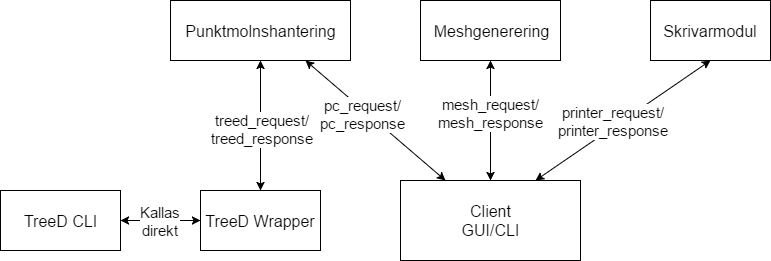
\includegraphics[width=130mm]{figures/Noddiagram.png}
	\caption{Diagram över ROS-noderna i första versionen av systemet}
	\label{fig:noddiagram}
\end{figure}

Det tänkta systemet kunde samla in fler punktmoln. Detta gjordes av punktmolnshanteringsnoden som tar in ett värde för hur noggrant objektet ska skannas. Punktmolnshanteringsnoden utför ett antal skanningar genom att noden TreeD-wrapper kallas. Sedan registrerar punktmolnshanteringsnoden dessa inkompletta punktmoln till ett punktmoln som representerar hela objektet.

När ett komplett punktmoln har genererats skickas det vidare till meshgenereringsnoden som uppskattar en tredimensionell yta, även kallad mesh, bestående av polygoner utifrån punktmolnet. Denna mesh kan sedan användas för att generera kod som kan köras på en 3D-skrivare för att skriva ut objektet.

Mycket tid under de första iterationerna av projektet spenderades på att utforska och undersöka olika tekniker och algoritmer. Som resultat av det finns det mycket nyttig kunskap i projektgruppen och även en del testkod för att utföra olika delar. Testkoden kommer till stor del kunna användas som utgångspunkt för det riktiga systemet.

Det ROS-baserade systemet var uppdelat i en serverdel och en klient. Tanken var att servern skulle köras på en dator som var fysiskt kopplad till hårdvaran och på så sätt kunde styra den genom TreeD-wrappern. Klienten skulle i första hand köras på samma dator och styra servern men med möjligheten att köras på en annan dator och styra servern över nätverket. Se figur \ref{fig:systembeskrivning_gamla} för en bild på hur det tänkta systemet var planerat att vara strukturerat.

\begin{figure}[H]
	\centering
	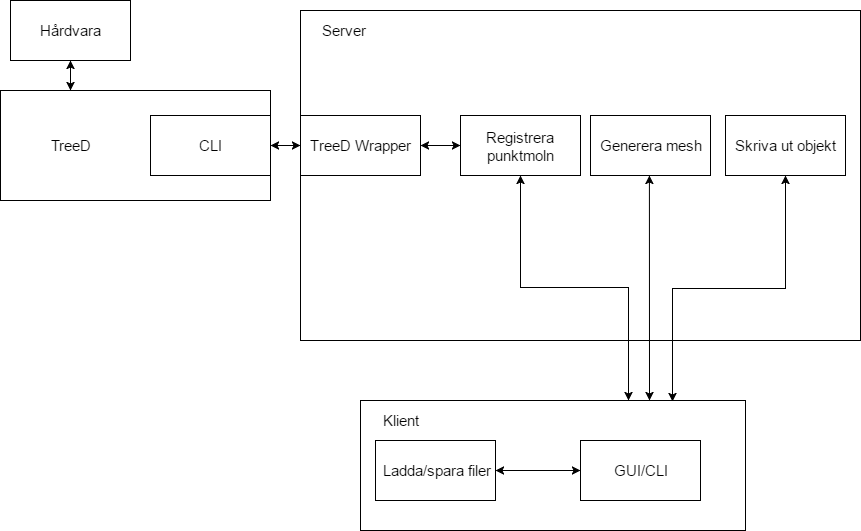
\includegraphics[width=130mm]{figures/Systemskiss_gamla.png}
	\caption{En skiss av det tänkta ROS-baserade systemet}
	\label{fig:systembeskrivning_gamla}
\end{figure}

Som kan ses i figurerna \ref{fig:systembeskrivning_gamla} och \ref{fig:noddiagram} så är klienten den centrala delen i programmet. Den hanterar användarens indata och använder sig av de olika noderna för att utföra de användaren vill. Konceptet var att systemet skulle använda en \textit{pipe and filter} arkitektur. Där klienten skickade runt data i pipen men att användaren, genom klienten hade möjlighet att granska resultatet och göra viss handpåläggning mellan de olika stegen. Detta genom att klienten alltid kan spara resultatet från ett steg till fil och använda andra program för handpåläggningen innan den skickas vidare i systemet.

\section{Systembeskrivning - 3D-Kopiering}

Som kan läsas tidigare i denna rapport så omförhandlades projektets krav och mål med kunden under projektets gång. Detta ledde till att gruppen gjorde om systemets arkitektur. ROS arkitekturen som presenterats ovan (se kap. 5.1) byttes ut mot att istället skapa ett objektorienterat program, skrivet i C++, som utför de operationer som behövs: registrering, filtrering och meshning. till detta program finns också ett CLI och ett GUI.

\subsection{Arkitektur}

\begin{figure}[H]
	\centering
	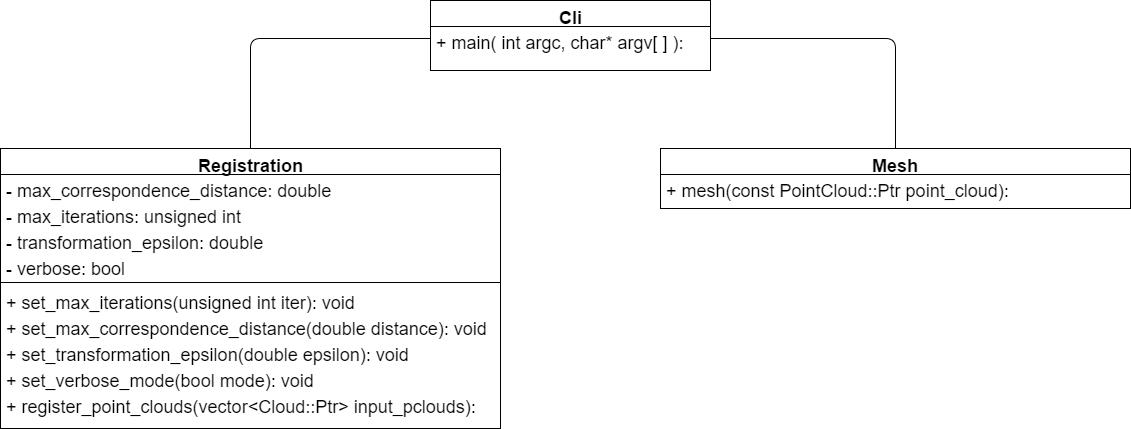
\includegraphics[width=130mm]{figures/klassdiagram.png}
	\caption{Översiktligt klassdiagram över arkitekturen}
	\label{fig:class_diagram}
\end{figure}

\subsection{Kommandoradsgränssnitt (CLI)}

Systemet kan kontrolleras av ett CLI som kan ta in olika parametrar för att anpassa registreringen. Det finns även alternativ för att bara registrera eller bara mesha objekt. När man kör programmet med hjälp av kommandoradsgränssnittet väljer man vilka filer eller mappar med filer programmet ska läsa in och använda. Hur de används beror på alternativen. Ett exempel på ett anrop är:\\\\
\textit{3DCopy -v --max-corr-dist 15 path/to/register/ output}\\\\
Det anropet kommer registrera och sedan mesha .pcd filerna i mappen path/to/register/ och döpa det kompletta punktmolnet respektive färdiga meshen till output.pcd och output.stl. Under registreringen och meshningen kommer programmet att skriva ut information om processen på grund av -v flaggan som står för \textit{verbose mode}. Om man undrar vilka alternativ som finns kan man använda -h flaggan så skriver programmet ut vilka alternativ som finns och hur man använder programmet med hjälp av kommandoradsgränssnittet. 

\subsection{GUI}
För att lättare kunna styra systemet utvecklades också ett GUI. GUI:t har nästintill samma funktionalitet som CLI:t och målet med att ha samma funktionalitet är att det inte ska spela någon roll om man använder CLI eller GUI.

\begin{figure}[H]
	\centering
	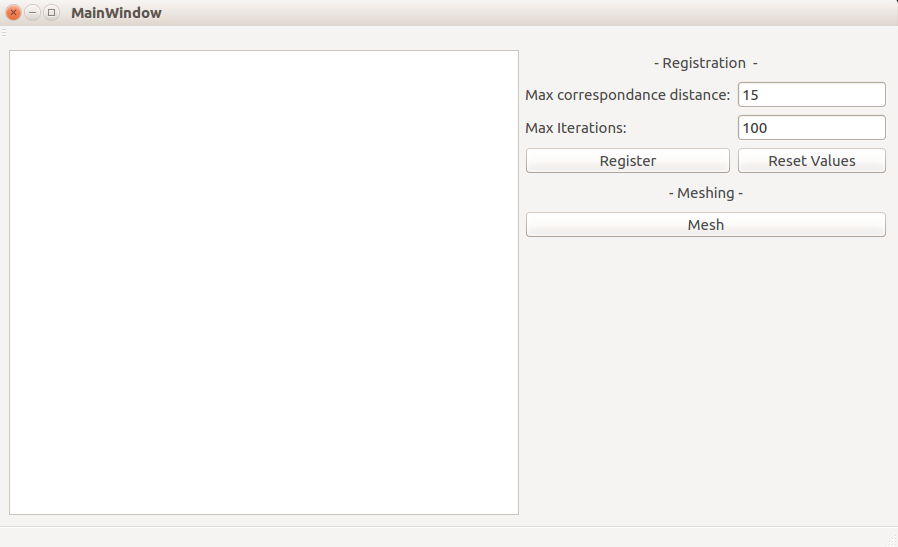
\includegraphics[width=130mm]{figures/3DCopyGUI.PNG}
	\caption{GUI:t för 3D-kopiering i slutet av iteration 2.}
	\label{fig:3dcopy_gui_res}
\end{figure}

De funktioner som finns i GUI:t just nu är Register som öppnar en dialog där man får välja en mapp som innehåller de punktmoln som man vill registrera. Det finns också en Mesh funktion där en dialog öppnas och man får välja det punktmoln som man vill mesha. Slutligen så finns det en funktion för att återställa parametervärdena för registreringen, Reset Values. De värden som återställs är Max correspondance distance och max iterations till 15 respektive 100.

\subsection{Meshning}

Den ytrekonstruering som systemet använder, PCLs Poisson surface reconstruction, är väldigt beroende av att det registrerade punktmolnet inte har några punkter som har hamnat fel. Om några punkter är fel eller det är för glest mellan punkterna så kan inte algoritmen räkna ut ytnormalerna korrekt. Om ytnormalerna blir fel så kommer inte meshen att stämma överens med det objekt som punktmolnet föreställer.

\begin{figure}[H]
	\centering
	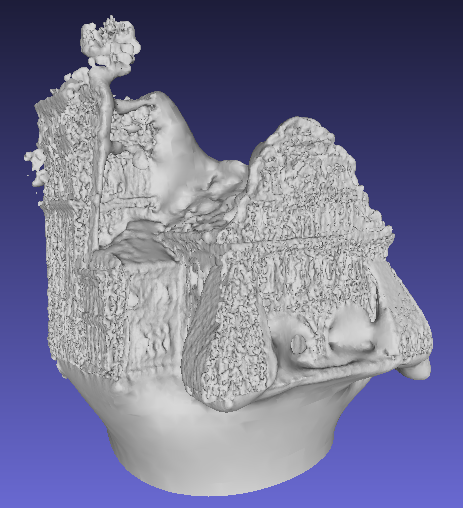
\includegraphics[width=80mm]{figures/3DCopyMeshChurch.PNG}
	\caption{Mesh av ofullständigt punktmoln som föreställer en kyrka.}
	\label{fig:3dcopy_mesh_church}
\end{figure}

I figur \ref{fig:3dcopy_mesh_church} kan man se var de olika problemen uppstår. Ovanpå och undertill kyrkan kan man se att det saknas punkter där det blir släta, rundade ytor som inte följer kanterna. Det syns också tydligt på flera ställen där meshen blir grynig att punkterna inte har hamnat rätt.

\section{Gemensamma erfarenheter}
%% Goda, mindre bra
%% I projektets alla faser
%% Tekniska, process-relaterade

I detta avsnitt presenteras de erfarenheter som gruppen har samlat på sig under projektets gång.

\subsection{Övergripande projekterfarenheter}

Att göra efterforskningar innan man börjar med någonting är väldigt viktigt och det märktes direkt i projektets början. Både genom att större delen av våra efterforskningar kom till stor hjälp direkt i projektet och bara några dagar in i första iterationen märktes det att det fanns några områden vi behövde läsa på mer om innan vi kunde skriva kod. Ett exempel på bra efterforskning som gjordes i förstudien var efterforskningarna kring ROS där alla gruppmedlemmar gick igenom tutorials och läste dokumentation som utvecklingsledaren gått igenom och tagit fram. I slutet av förstudien gjordes en gemensam kodutmaning där alla fick skriva varsin chattklient med hjälp av ROS. Kodutmaningen ledde till att alla kom in i ROS, Git, Python och andra verktyg som skulle användas under resten av projektet.


\subsection{Erfarenheter gällande kommunikation}

Betydelsen av kommunikation var stor under projektets gång. Verktygen Slack och Trello har använts flitigt och varit givande för gruppen. Med Slack har vi alltid kunnat nå varandra snabbt och smidigt. Vi har kunnat hålla informationsflöden skilda och sorterade i olika kanaler. Funktioner som påminnelser och trådar har också varit till stor hjälp för att lätt kunna komma åt den informationen som man vill åt i flödena. För att ha en översikt i hur det går med olika delar av projektet har man använt Trello. Genom att ha olika listor för statusen av dokument och funktioner under utveckling har gjort att man som gruppmedlem lätt kunnat se hur det går och vad man behöver göra. 


\subsection{Erfarenheter gällande kvalité}

Kvalité har varit viktigt för gruppen och kvalitetsansvarig har gjort ett bra jobb med att se till att projektets kod och dokument håller en hög standard. Detta framförallt genom granskning av dokument och kod. All kod i projektet har genomgått granskning för att säkerställa god kvalité. Till detta har Githubs pull request-funktion använts där alla gruppmedlemmar kunnat kommentera och diskutera koden innan den går in i master branchen hos repositoriet. Dokumenten har också granskats, då genom korrekturläsning. All denna granskning har varit mycket bra för att se hur andra skriver dokument och kod.

\subsection{Erfarenheter av att bygga vidare på ett projekt}

I mitten av projektet upptäckte gruppen att det system som skulle vidareutvecklas inte fungerade tillräckligt stabilt för att det skulle vara möjligt att integrera med det system som gruppen utvecklade. Gruppen litade på att kunden hade god insikt i det tidigare systemet och eftersom att dessa fel inte togs upp i början av projektet förutsatte gruppen att det tidigare systemet inte innehöll några fel.

Eftersom att gruppen inte hade någon anledning att tro att det tidigare systemet innehöll fel så genomfördes ingen rigorös testning av det tidigare systemet. Det saknades också testdokumentation och  annan dokumentation från den grupp som hade utvecklat det tidigare systemet. Det visar vikten av att väl dokumentera sitt system för att undvika problem i framtiden.


\section{Översikt över individuella bidrag}

Här listas de individuella bidrag som gruppens medlemmar har bidragit med till rapporten:

\begin{itemize}
	\item Dunström, Hampus - Hur påverkas ett team av sin arbetsmiljö?
	\item Holmberg, Olof - Kontexters påverkan vid testning av GUI
	\item Jannering, Gustav - Hur kravhanteringsmetoder påverkar ett utvecklingsprojekt
	\item Karlsson, Michael - Analys av punktmolnsregistrering
	\item Lundberg, Martin - Att bygga ett system i ROS
	\item Tuhkala, Hannes - Att använda sig av \latex för större dokument
	\item Wallström, Fredrik - Kvalitetsarbete i praktiken
\end{itemize}


%%%%%%%%%%%%%%%%%%%%%%%%%%%%%%%%%%%%%%%%%%%%%%%%%%%%%%%%%%%%%%%%%%%%%%
%%% results.tex ends here